\documentclass[14pt]{article}

\usepackage{amsmath}
\usepackage{amssymb}
\usepackage{amsthm}
\usepackage{geometry,enumerate}
\usepackage{tikz}
\usetikzlibrary{positioning, arrows, automata}
\usepackage{graphicx}
\usepackage{xcolor}
\usepackage{enumitem}
\geometry{margin=25mm}
\usepackage{hyperref}
\hypersetup{
    colorlinks=true,
    linkcolor=blue,
    filecolor=magenta,      
    urlcolor=cyan,
}
\urlstyle{same}

\usepackage{ulem}
\usepackage{cancel}
\usepackage{comment}
\usepackage[parfill]{parskip}

\newcommand\heightA{0.5in}
\newcommand\heightB{1.0in}


\title{\textbf{10-417 Final Project Proposal}
\\{\Large Numerically Solving PDEs using Deep Neural Networks}}
\author{Alex Havrilla \& Alden Pritchard}

\begin{document}
\maketitle


\section{ Statement of Purpose }

Our goal is to numerically solve a specific class of quasi-linear Partial Differential Equations (PDEs) using a deep neural network. In practice, it takes a lot of effort to solve just one very well, so we must develop good methods to solve even one very well with DGM because there are several matters to consider, such as the DGM Architecture, neural network parameters, interior point sampling method, neural network size, and more. 
So, we will start by trying to solve the heat equation as this will be a good proof on concept. Once we’ve done this we’ll move on to harder equations (we’ll pick these later). Once we do this, we can think about solving not just PDEs, but also arbitrary functions, such as the Ray-Tracing equation (may not get this far).

\section{ Motivation }

Standard methods for solving PDEs include Euler steps, Runge-Kutta, Galerkin methods, etc. Short description here. The high level idea is that these methods mesh the domain in which we want to solve the PDE and then take small steps to solve the PDE. However, as the dimension increases, the number of steps grows exponentially, making this process infeasible. This leaves us with a lack of good methods for solving PDEs in higher dimensional spaces.

\section{ Advantages of Deep Galerkin Method }

First proposed in 2018 by \_\_\_\_ and \_\_\_\_. They used the DGM to numerically solve the Black-Scholes equation (a well-studied PDE that has many important uses in finance, but also has no analytical solution). This main advantage of this method is that it is mesh-free, and as a result does not suffer from the curse of dimensionality, which allows us to compute values in feasible time. These authors proved rigorously that using a deep neural network, as the number of layers goes to infinity, the network approximation converges point wise to the true solution. The way this is done is that we have a loss function which comprises of distance from initial condition, distance from boundary condition, and distance from the size of the differential operator applied to the function. So, if we minimize these three terms, we get a neural network which has output closely approximating the boundary conditions and also closely approximates a solution on the interior of the domain.
\newpage
\begin{center}
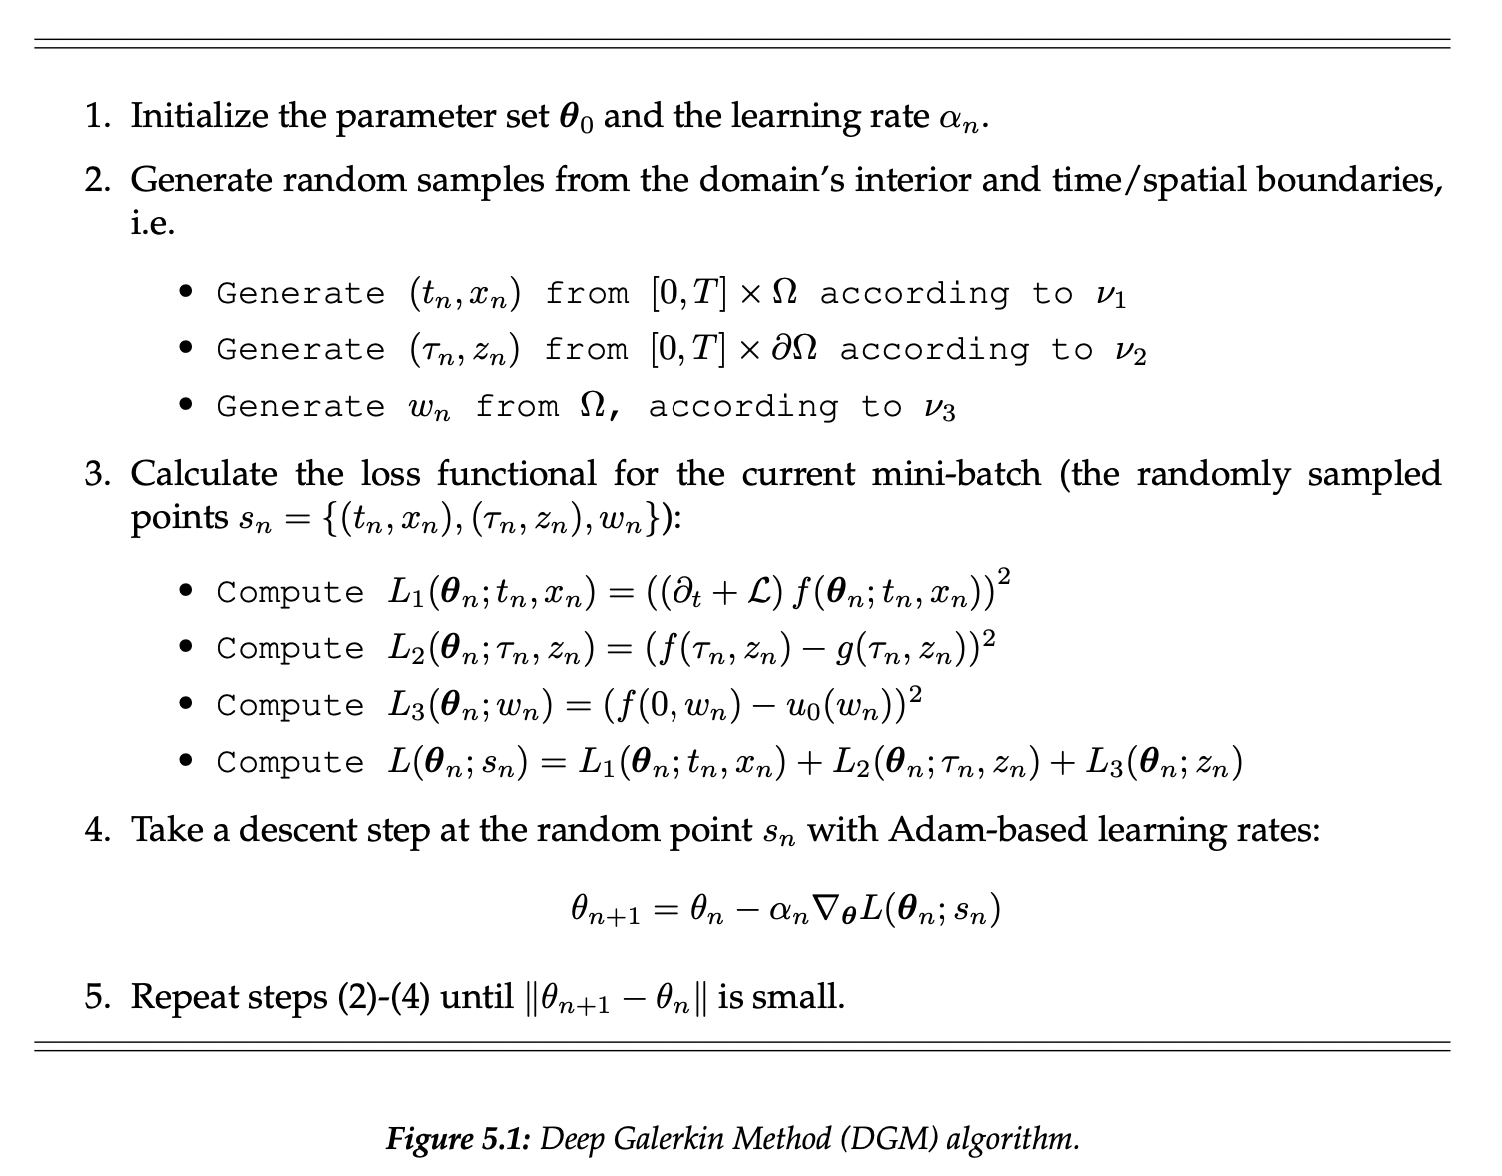
\includegraphics[scale=0.5]{DGM_Algorithm.png}
\end{center}\\
Short description

\section{ Implementation Details }

\subsection{ Overall Architecture }\\
\begin{center}
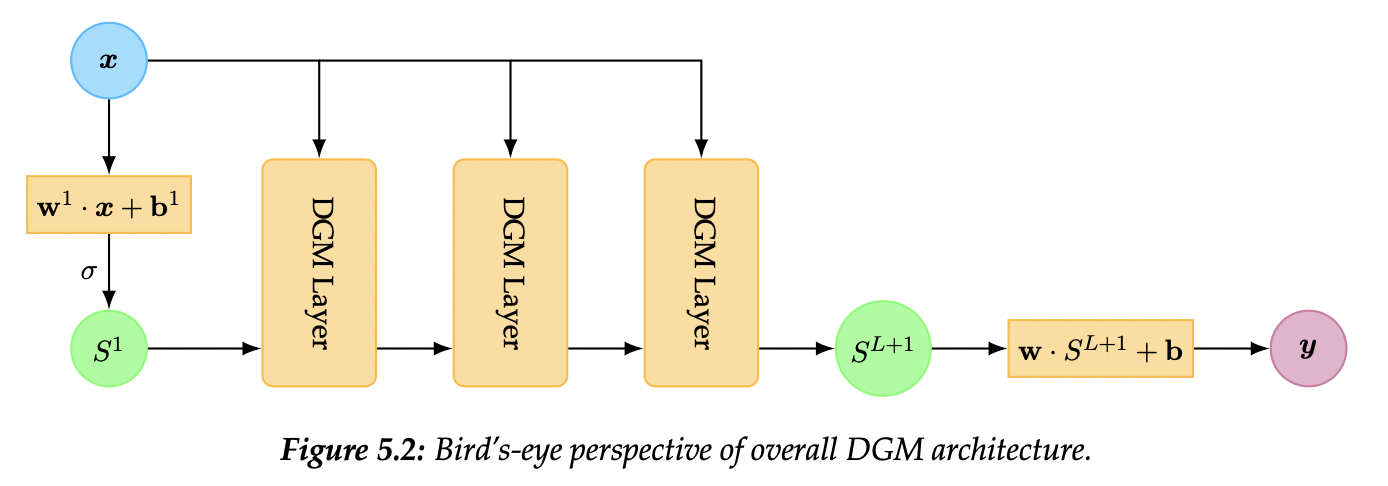
\includegraphics[scale=0.5]{Architecture.png}
\end{center}\\
The overall architecture consists of series of layers of DGM layers that take as input the original x and the output of the previous DGM layer (add why this makes sense), as well as two linear layers, one at the start and one at the end.


\subsection{ Individual DGM layer }
\\\begin{center}
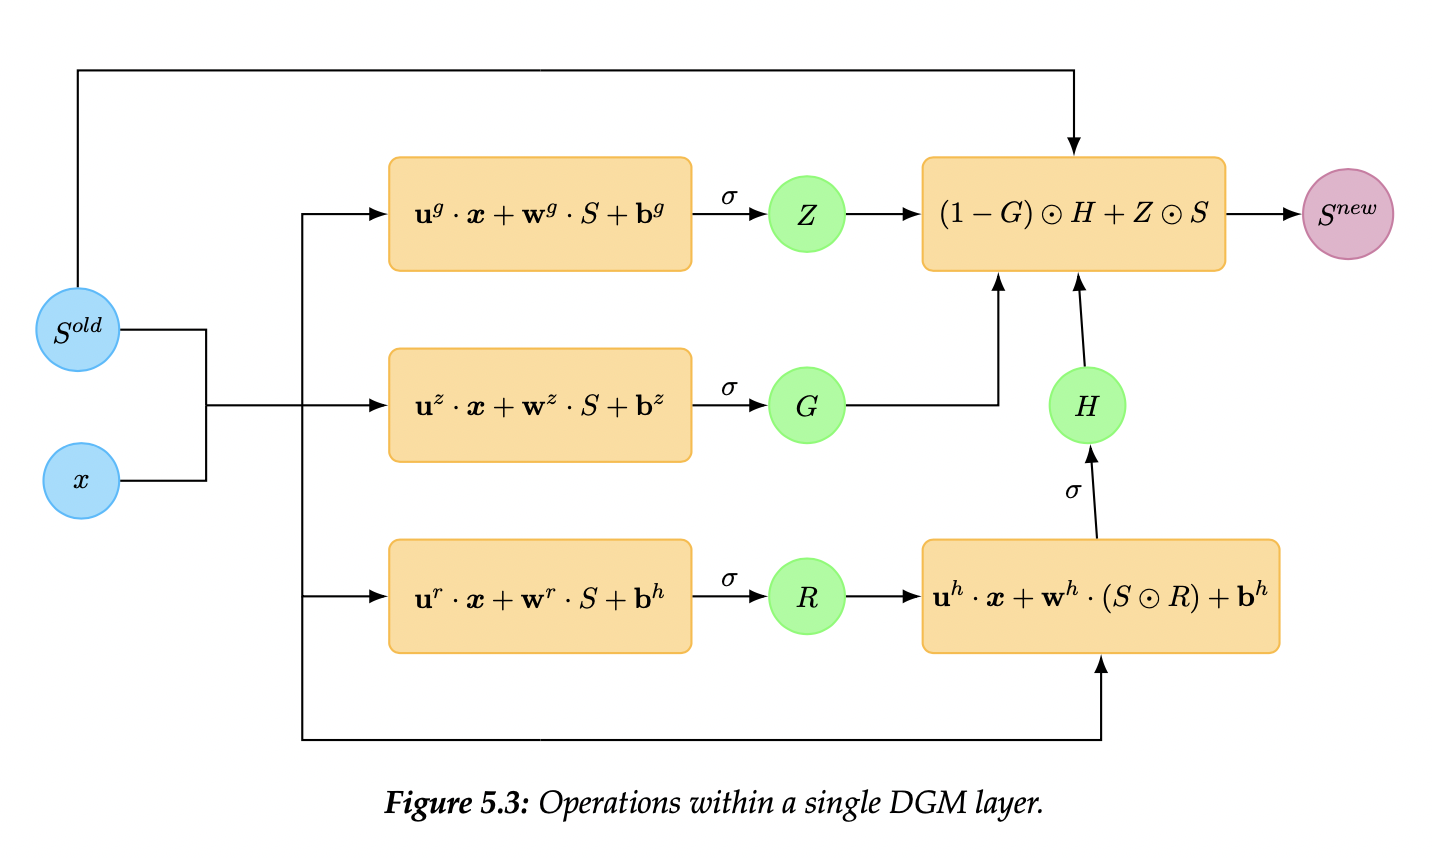
\includegraphics[scale=0.5]{DGM_Layer.png}
\end{center}\\
The individual DGM layer consists of four sums of linear maps and an output function. Each DGM layer consists of eight weight matrices, four bias vectors, and four activation functions which are combined in the output function.

\section{ Room for Improvement }
Some PDEs involve second or higher order derivatives. One way to compute these is to use back propagation, but this is quadratic in the dimension of the input variables. The authors avoided using backpropagation by using a finite difference method. We believe there is room for improvement here in the finite difference approximation used. There are also questions of sampling methodologies and which distributions are most appropriate for each equation. There are also considerations regarding network structure and computation time where we anticipate having lots of different things to try. Lastly, it is a lot of effort to solve even a single PDE well is valuable, so we believe even approximating one PDE well will be a significant contribution.

\end{document}
